\documentclass[a4paper]{article}

\def\npart {III}
\def\nterm {Michaelmas}
\def\nyear {2017}
\def\nlecturer {M. Lis}
\def\ncourse {Advanced Probability}

% Imports
\ifx \nextra \undefined
  \usepackage[pdftex,
    hidelinks,
    pdfauthor={Dexter Chua},
    pdfsubject={Cambridge Maths Notes: Part \npart\ - \ncourse},
    pdftitle={Part \npart\ - \ncourse},
  pdfkeywords={Cambridge Mathematics Maths Math \npart\ \nterm\ \nyear\ \ncourse}]{hyperref}
  \title{Part \npart\ - \ncourse}
\else
  \usepackage[pdftex,
    hidelinks,
    pdfauthor={Dexter Chua},
    pdfsubject={Cambridge Maths Notes: Part \npart\ - \ncourse\ (\nextra)},
    pdftitle={Part \npart\ - \ncourse\ (\nextra)},
  pdfkeywords={Cambridge Mathematics Maths Math \npart\ \nterm\ \nyear\ \ncourse\ \nextra}]{hyperref}

  \title{Part \npart\ - \ncourse \\ {\Large \nextra}}
\fi

\author{Lectured by \nlecturer \\\small Notes taken by Dexter Chua}
\date{\nterm\ \nyear}

\usepackage{alltt}
\usepackage{amsfonts}
\usepackage{amsmath}
\usepackage{amssymb}
\usepackage{amsthm}
\usepackage{booktabs}
\usepackage{caption}
\usepackage{enumitem}
\usepackage{fancyhdr}
\usepackage{graphicx}
\usepackage{mathtools}
\usepackage{microtype}
\usepackage{multirow}
\usepackage{pdflscape}
\usepackage{pgfplots}
\usepackage{siunitx}
\usepackage{tabularx}
\usepackage{tikz}
\usepackage{tkz-euclide}
\usepackage[normalem]{ulem}
\usepackage[all]{xy}

\pgfplotsset{compat=1.12}

\pagestyle{fancyplain}
\lhead{\emph{\nouppercase{\leftmark}}}
\ifx \nextra \undefined
  \rhead{
    \ifnum\thepage=1
    \else
      \npart\ \ncourse
    \fi}
\else
  \rhead{
    \ifnum\thepage=1
    \else
      \npart\ \ncourse\ (\nextra)
    \fi}
\fi
\usetikzlibrary{arrows}
\usetikzlibrary{decorations.markings}
\usetikzlibrary{decorations.pathmorphing}
\usetikzlibrary{positioning}
\usetikzlibrary{fadings}
\usetikzlibrary{intersections}
\usetikzlibrary{cd}

\newcommand*{\Cdot}{\raisebox{-0.25ex}{\scalebox{1.5}{$\cdot$}}}
\newcommand {\pd}[2][ ]{
  \ifx #1 { }
    \frac{\partial}{\partial #2}
  \else
    \frac{\partial^{#1}}{\partial #2^{#1}}
  \fi
}

% Theorems
\theoremstyle{definition}
\newtheorem*{aim}{Aim}
\newtheorem*{axiom}{Axiom}
\newtheorem*{claim}{Claim}
\newtheorem*{cor}{Corollary}
\newtheorem*{defi}{Definition}
\newtheorem*{eg}{Example}
\newtheorem*{fact}{Fact}
\newtheorem*{law}{Law}
\newtheorem*{lemma}{Lemma}
\newtheorem*{notation}{Notation}
\newtheorem*{prop}{Proposition}
\newtheorem*{thm}{Theorem}

\renewcommand{\labelitemi}{--}
\renewcommand{\labelitemii}{$\circ$}
\renewcommand{\labelenumi}{(\roman{*})}

\let\stdsection\section
\renewcommand\section{\newpage\stdsection}

% Strike through
\def\st{\bgroup \ULdepth=-.55ex \ULset}

% Maths symbols
\newcommand{\bra}{\langle}
\newcommand{\ket}{\rangle}

\newcommand{\N}{\mathbb{N}}
\newcommand{\Z}{\mathbb{Z}}
\newcommand{\Q}{\mathbb{Q}}
\renewcommand{\H}{\mathbb{H}}
\newcommand{\R}{\mathbb{R}}
\newcommand{\C}{\mathbb{C}}
\newcommand{\Prob}{\mathbb{P}}
\renewcommand{\P}{\mathbb{P}}
\newcommand{\E}{\mathbb{E}}
\newcommand{\F}{\mathbb{F}}
\newcommand{\cU}{\mathcal{U}}
\newcommand{\RP}{\mathbb{RP}}
\newcommand{\CP}{\mathbb{CP}}

\newcommand{\ph}{\,\cdot\,}

\DeclareMathOperator{\sech}{sech}
\DeclareMathOperator{\cosech}{cosech}
\DeclareMathOperator{\cosec}{cosec}

\DeclareMathOperator{\covol}{covol}
\DeclareMathOperator{\vol}{vol}

\let\Im\relax
\let\Re\relax
\DeclareMathOperator{\Im}{Im}
\DeclareMathOperator{\Re}{Re}
\DeclareMathOperator{\im}{im}
\DeclareMathOperator{\image}{image}
\DeclareMathOperator{\Ann}{Ann}

\DeclareMathOperator*{\res}{res}
\DeclareMathOperator{\Res}{Res}
\DeclareMathOperator{\Ind}{Ind}

\DeclareMathOperator{\tr}{tr}
\DeclareMathOperator{\diag}{diag}
\DeclareMathOperator{\rank}{rank}
\DeclareMathOperator{\card}{card}
\DeclareMathOperator{\spn}{span}
\DeclareMathOperator{\adj}{adj}

\DeclareMathOperator{\erf}{erf}
\DeclareMathOperator{\erfc}{erfc}

\DeclareMathOperator{\ord}{ord}
\DeclareMathOperator{\Sym}{Sym}

\DeclareMathOperator{\sgn}{sgn}
\DeclareMathOperator{\orb}{orb}
\DeclareMathOperator{\stab}{stab}
\DeclareMathOperator{\ccl}{ccl}

\DeclareMathOperator{\lcm}{lcm}
\DeclareMathOperator{\hcf}{hcf}

\DeclareMathOperator{\Int}{Int}
\DeclareMathOperator{\id}{id}

\DeclareMathOperator{\betaD}{beta}
\DeclareMathOperator{\gammaD}{gamma}
\DeclareMathOperator{\Poisson}{Poisson}
\DeclareMathOperator{\binomial}{binomial}
\DeclareMathOperator{\multinomial}{multinomial}
\DeclareMathOperator{\Bernoulli}{Bernoulli}
\DeclareMathOperator{\like}{like}

\DeclareMathOperator{\var}{var}
\DeclareMathOperator{\cov}{cov}
\DeclareMathOperator{\bias}{bias}
\DeclareMathOperator{\mse}{mse}
\DeclareMathOperator{\corr}{corr}

\DeclareMathOperator{\otp}{otp}
\DeclareMathOperator{\dom}{dom}

\DeclareMathOperator{\Root}{Root}
\DeclareMathOperator{\supp}{supp}
\DeclareMathOperator{\rel}{rel}
\DeclareMathOperator{\Hom}{Hom}
\DeclareMathOperator{\Aut}{Aut}
\DeclareMathOperator{\Gal}{Gal}
\DeclareMathOperator{\Mat}{Mat}
\DeclareMathOperator{\End}{End}
\DeclareMathOperator{\Char}{char}
\DeclareMathOperator{\ev}{ev}
\DeclareMathOperator{\St}{St}
\DeclareMathOperator{\Lk}{Lk}
\DeclareMathOperator{\disc}{disc}
\DeclareMathOperator{\Isom}{Isom}
\DeclareMathOperator{\length}{length}
\DeclareMathOperator{\energy}{energy}
\DeclareMathOperator{\area}{area}
\DeclareMathOperator{\Syl}{Syl}
\DeclareMathOperator{\cl}{cl}
\DeclareMathOperator{\fix}{fix}

\newcommand{\GL}{\mathrm{GL}}
\newcommand{\SL}{\mathrm{SL}}
\newcommand{\PGL}{\mathrm{PGL}}
\newcommand{\PSL}{\mathrm{PSL}}
\newcommand{\PSU}{\mathrm{PSU}}
\newcommand{\Or}{\mathrm{O}}
\newcommand{\SO}{\mathrm{SO}}
\newcommand{\U}{\mathrm{U}}
\newcommand{\SU}{\mathrm{SU}}

\renewcommand{\d}{\mathrm{d}}
\newcommand{\D}{\mathrm{D}}

\tikzset{->/.style = {decoration={markings,
                                  mark=at position 1 with {\arrow[scale=2]{latex'}}},
                      postaction={decorate}}}
\tikzset{<-/.style = {decoration={markings,
                                  mark=at position 0 with {\arrowreversed[scale=2]{latex'}}},
                      postaction={decorate}}}
\tikzset{<->/.style = {decoration={markings,
                                   mark=at position 0 with {\arrowreversed[scale=2]{latex'}},
                                   mark=at position 1 with {\arrow[scale=2]{latex'}}},
                       postaction={decorate}}}
\tikzset{->-/.style = {decoration={markings,
                                   mark=at position #1 with {\arrow[scale=2]{latex'}}},
                       postaction={decorate}}}
\tikzset{-<-/.style = {decoration={markings,
                                   mark=at position #1 with {\arrowreversed[scale=2]{latex'}}},
                       postaction={decorate}}}

\tikzset{circ/.style = {fill, circle, inner sep = 0, minimum size = 3}}
\tikzset{mstate/.style={circle, draw, blue, text=black, minimum width=0.7cm}}

\definecolor{mblue}{rgb}{0.2, 0.3, 0.8}
\definecolor{morange}{rgb}{1, 0.5, 0}
\definecolor{mgreen}{rgb}{0.1, 0.4, 0.2}
\definecolor{mred}{rgb}{0.5, 0, 0}

\def\drawcirculararc(#1,#2)(#3,#4)(#5,#6){%
    \pgfmathsetmacro\cA{(#1*#1+#2*#2-#3*#3-#4*#4)/2}%
    \pgfmathsetmacro\cB{(#1*#1+#2*#2-#5*#5-#6*#6)/2}%
    \pgfmathsetmacro\cy{(\cB*(#1-#3)-\cA*(#1-#5))/%
                        ((#2-#6)*(#1-#3)-(#2-#4)*(#1-#5))}%
    \pgfmathsetmacro\cx{(\cA-\cy*(#2-#4))/(#1-#3)}%
    \pgfmathsetmacro\cr{sqrt((#1-\cx)*(#1-\cx)+(#2-\cy)*(#2-\cy))}%
    \pgfmathsetmacro\cA{atan2(#2-\cy,#1-\cx)}%
    \pgfmathsetmacro\cB{atan2(#6-\cy,#5-\cx)}%
    \pgfmathparse{\cB<\cA}%
    \ifnum\pgfmathresult=1
        \pgfmathsetmacro\cB{\cB+360}%
    \fi
    \draw (#1,#2) arc (\cA:\cB:\cr);%
}
\newcommand\getCoord[3]{\newdimen{#1}\newdimen{#2}\pgfextractx{#1}{\pgfpointanchor{#3}{center}}\pgfextracty{#2}{\pgfpointanchor{#3}{center}}}

\def\Xint#1{\mathchoice
   {\XXint\displaystyle\textstyle{#1}}%
   {\XXint\textstyle\scriptstyle{#1}}%
   {\XXint\scriptstyle\scriptscriptstyle{#1}}%
   {\XXint\scriptscriptstyle\scriptscriptstyle{#1}}%
   \!\int}
\def\XXint#1#2#3{{\setbox0=\hbox{$#1{#2#3}{\int}$}
     \vcenter{\hbox{$#2#3$}}\kern-.5\wd0}}
\def\ddashint{\Xint=}
\def\dashint{\Xint-}


% Example Sheets -- on James Norris website, latest friday before, W/X pigeon hole, Mo Dick Wong, mdw46
% 1: 1.3, 2.3
% 2: 3.8, 3.10
% 3: 6.1, 7.4
% 4: 7.10, 9.2

\pgfdeclaredecoration{penciline}{initial}{
    \state{initial}[width=+\pgfdecoratedinputsegmentremainingdistance,auto corner on length=1mm,]{
        \pgfpathcurveto%
        {% From
            \pgfqpoint{\pgfdecoratedinputsegmentremainingdistance}
                            {\pgfdecorationsegmentamplitude}
        }
        {%  Control 1
        \pgfmathrand
        \pgfpointadd{\pgfqpoint{\pgfdecoratedinputsegmentremainingdistance}{0pt}}
                        {\pgfqpoint{-\pgfdecorationsegmentaspect\pgfdecoratedinputsegmentremainingdistance}%
                                        {\pgfmathresult\pgfdecorationsegmentamplitude}
                        }
        }
        {%TO
        \pgfpointadd{\pgfpointdecoratedinputsegmentlast}{\pgfpoint{1pt}{1pt}}
        }
    }
    \state{final}{}
}

\begin{document}
\maketitle
{\small
\setlength{\parindent}{0em}
\setlength{\parskip}{1em}

The aim of the course is to introduce students to advanced topics in modern probability theory. The emphasis is on tools required in the rigorous analysis of stochastic processes, such as Brownian motion, and in applications where probability theory plays an important role.

\noindent\textbf{Review of measure and integration:} sigma-algebras, measures and filtrations; integrals and expectation; convergence theorems; product measures, independence and Fubini's theorem.\\
\noindent\textbf{Conditional expectation:} Discrete case, Gaussian case, conditional density functions; existence and uniqueness; basic properties.\\
\noindent\textbf{Martingales:} Martingales and submartingales in discrete time; optional stopping; Doob's inequalities, upcrossings, martingale convergence theorems; applications of martingale techniques.\\
\noindent\textbf{Stochastic processes in continuous time:} Kolmogorov's criterion, regularization of paths; martingales in continuous time.\\
\noindent\textbf{Weak convergence:} Definitions and characterizations; convergence in distribution, tightness, Prokhorov's theorem; characteristic functions, L\'evy's continuity theorem.\\
\noindent\textbf{Sums of independent random variables:} Strong laws of large numbers; central limit theorem; Cram\'er's theory of large deviations.\\
\noindent\textbf{Brownian motion:} Wiener's existence theorem, scaling and symmetry properties; martingales associated with Brownian motion, the strong Markov property, hitting times; properties of sample paths, recurrence and transience; Brownian motion and the Dirichlet problem; Donsker's invariance principle.\\
\noindent\textbf{Poisson random measures:} Construction and properties; integrals.\\
\noindent\textbf{L\'evy processes:} L\'evy-Khinchin theorem.

\subsubsection*{Pre-requisites}
A basic familiarity with measure theory and the measure-theoretic formulation of probability theory is very helpful. These foundational topics will be reviewed at the beginning of the course, but students unfamiliar with them are expected to consult the literature (for instance, Williams' book) to strengthen their understanding.
}
\tableofcontents

\section{Introduction}
In some other places in the world, this course might be known as ``Stochastic Processes''. In addition to doing probability, a new component studied in the course is \emph{time}. We are going to study how things change over time.

In the first half of the course, we will focus on discrete time. We will have a discrete sequence of points, and we assign some random values to each of these points. The point, of course, is that there will be dependencies between the different points.

In the second half of the course, we will look at continuous time. There is a fundamental difference between the two, in that there is a nice topology on the interval. This allows us to say things like we want our trajectories to be continuous. However, we will see that to understand continuous time, we start with the corresponding discrete situation, and then try to ``take the limit'' as the sample points become closer and closer to each other. An important example is Brownian motion.

There are two main objects that appear in this course. The first is the conditional expectation. Recall that if we have a random variable $X$, we can obtain a number $\E[X]$, the expectation of $X$. We can think of this as integrating out all the randomness of the system. Conditional expectation will be some subtle modification of this construction, where we don't actually get a number, but another random variable. The idea behind this is that we want to integrate out some of the randomness in our random variable.

Another main object is \emph{stopping time}. For example, if we have a production line that produces random number of outputs at each point, then we can ask how much time it takes to produce a fixed number of goods, and this is a nice random time, which we call a stopping time. The niceness follows from the fact that if the time comes, we know it. An example that is not nice is, for example, the last day it rains in Cambridge in a particular month, since on that last day, we don't necessarily know that it is in fact the last day.

\section{Some measure theory}
\subsection{Review of measure theory}
To make the course as self-contained as possible, we shall begin with some review of measure theory. On the other hand, if one doesn't already know measure theory, they are recommended to learn the measure theory properly before starting this course.

\begin{defi}[$\sigma$-algebra]\index{$\sigma$-algebra}
  Let $E$ be a set. A subset $\mathcal{E}$ of the power set $\mathcal{P}(E)$ is called a \emph{$\sigma$-algebra} (or \term{$\sigma$-field}) if
  \begin{enumerate}
    \item $\emptyset \in \mathcal{E}$;
    \item If $A \in \mathcal{E}$, then $A^C = E \setminus A \in \mathcal{E}$;
    \item If $A_1, A_2, \ldots \in \mathcal{E}$, then $\bigcup_{n = 1}^\infty A_n \in \mathcal{E}$.
  \end{enumerate}
\end{defi}

\begin{defi}[Measurable space]\index{measurable space}
  A \emph{measurable space} is a set with a $\sigma$-algebra.
\end{defi}


\begin{defi}[Borel $\sigma$-algebra]\index{Borel $\sigma$-algebra}\index{$\sigma$-algebra!Borel}\index{$\mathcal{B}(E)$}
  Let $E$ be a topological space with topology $\mathcal{T}$. Then the \emph{Borel $\sigma$-algebra} $\mathcal{B}(E)$ on $E$ is the $\sigma$-algebra generated by $\mathcal{T}$, i.e.\ the smallest $\sigma$-algebra containing $\mathcal{T}$.
\end{defi}

We are often going to look at $\mathcal{B}(\R)$, and we will just write $\mathcal{B}$\index{$\mathcal{B}$} for it.

\begin{defi}[Measure]\index{measure}
  A function $\mu: \mathcal{E} \to [0, \infty]$ is a \emph{measure} if
  \begin{itemize}
    \item $\mu(\emptyset) = 0$
    \item If $A_1, A_2, \ldots \in \mathcal{E}$ are disjoint, then
      \[
        \mu \left(\bigcup_{i = 1}^\infty A_i \right) = \sum_{i = 1}^\infty \mu(A_i).
      \]
  \end{itemize}
\end{defi}

\begin{defi}[Measure space]\index{measure space}
  A \emph{measure space} is a measurable space with a measure.
\end{defi}

\begin{defi}[Measurable function]\index{measurable function}
  Let $(E_1, \mathcal{E}_1)$ and $(E_2, \mathcal{E}_2)$ be measurable spaces. Then $f: E_1 \to E_2$ is said to be \emph{measurable} if $A \in \mathcal{E}_2$ implies $f^{-1}(A) \in \mathcal{E}_1$.
\end{defi}
This is similar to the definition of a continuous function.

\begin{notation}\index{$m\mathcal{E}$}\index{$m\mathcal{E}^+$}
  For $(E, \mathcal{E})$ a measurable space, we write $m\mathcal{E}$ for the set of measurable functions $E \to \R$.

  We write $m\mathcal{E}^+$ to be the positive measurable functions, which are allowed to take value $\infty$.
\end{notation}
Note that we do \emph{not} allow taking the values $\pm \infty$ in the first case.

\begin{thm}
  Let $(E, \mathcal{E}, \mu)$ be a measure space. Then there exists a unique function $\tilde{\mu}: m\mathcal{E}^+ \to [0, \infty]$ satisfying
  \begin{itemize}
    \item $\tilde{\mu}(\mathbf{1}_A) = \mu(A)$, where $\mathbf{1}_A$ is the indicator function of $A$.
    \item Linearity: $\tilde{\mu}(\alpha f + \beta g) = \alpha \tilde{\mu}(f) + \beta \tilde{\mu}(g)$ if $\alpha, \beta \in \R_{\geq 0}$ and $f, g \in m\mathcal{E}^+$.
    \item Monotone convergence: iff $f_1, f_2, \ldots \in m\mathcal{E}^+$ are such that $f_n \nearrow f \in m\mathcal{E}^+$ pointwise a.e.\ as $n \to \infty$, then
      \[
        \lim_{n \to \infty} \tilde{\mu}(f_n) = \tilde{\mu} (f).
      \]
  \end{itemize}
  We call $\tilde{\mu}$ the \term{integral} with respect to $\mu$, and we will write it as $\mu$ from now on.
\end{thm}

\begin{defi}[Simple function]\index{simple function}
  A function $f$ is \emph{simple} if there exists $\alpha_n \in \R_{\geq 0}$ and $A_n \in \mathcal{E}$ for $1 \leq n \leq k$ such that
  \[
    f = \sum_{n = 1}^k \alpha_n \mathbf{1}_{A_n}.
  \]
\end{defi}
From the first two properties of the measure, we see that
\[
  \mu(f) = \sum_{n = 1}^k \alpha_n \mu(A_n).
\]
One convenient observation is that a function is simple iff it takes on only finitely many values. We then see that if $f \in m \mathcal{E}^+$, then
\[
  f_n = 2^{-n}\lfloor 2^n f\rfloor \wedge n
\]
is a sequence of simple functions approximating $f$ from below. Thus, given monotone convergence, this shows that
\[
  \mu(f) = \lim \mu(f_n),
\]
and this proves the uniqueness part of the theorem.

Recall that
\begin{defi}[Almost everywhere]\index{almost everywhere}
  We say $f = g$ almost everywhere if
  \[
    \mu(\{x \in E: f(x) \not= g(x)\}) = 0.
  \]
  We say $f$ is a \term{version} of $g$.
\end{defi}

\begin{eg}
  Let $\ell_n = \mathbf{1}_{[n, n + 1]}$. Then $\mu(\ell_n) = 1$ for all $1$, but also $f_n \to 0$ and $\mu(0) = 0$. So the ``monotone'' part of monotone convergence is important.
\end{eg}

So if the sequence is not monotone, then the measure does not preserve limits, but it turns out we still have an inequality.

\begin{lemma}[Fatou's lemma]\index{Fatou's lemma}
  Let $f_i \in m \mathcal{E}^+$. Then
  \[
    \mu\left(\liminf_n f_n\right) \leq \liminf_n \mu(f_n).
  \]
\end{lemma}

\begin{proof}
  Apply monotone convergence to the sequence $\inf_{m \geq n} f_m$
\end{proof}

Of course, it would be useful to extend integration to functions that are not necessarily positive.
\begin{defi}[Integrable function]\index{integrable function}
  We say a function $f \in m\mathcal{E}$ is \emph{integrable} if $\mu(|f|) \leq \infty$. We write \term{$L^1(E)$} (or just $L^1$) for the space of integrable functions.

  We extend $\mu$ to $L^1$ by
  \[
    \mu(f) = \mu(f^+) - \mu(f^-),
  \]
  where $f^{\pm} = (\pm f) \wedge 0$.
\end{defi}

If we want to be explicit about the measure and the $\sigma$-algebra, we can write $L^1(E, \mathcal{E} \mu)$.

\begin{thm}[Dominated convergence theorem]\index{dominated convergence theorem}
  If $f_i \in m\mathcal{E}$ and $f_i \to f$ a.e., such that there exists $g \in L^1$ such that $|f_i| \leq g$ a.e. Then
  \[
    \mu(f) = \lim \mu(f_n).
  \]
\end{thm}

\begin{proof}
  Apply Fatou's lemma to $g - f_n$ and $g + f_n$.
\end{proof}

\begin{defi}[Product $\sigma$-algebra]\index{product $\sigma$-algebra}\index{$\sigma$-algebra!product}
  Let $(E_1, \mathcal{E}_1)$ and $(E_2 , \mathcal{E}_2)$ be measure spaces. Then the product $\sigma$-algebra$ \mathcal{E}_1 \otimes \mathcal{E}_2$ is the smallest $\sigma$-algebra on $E_1 \times E_2$ containing all sets of the form $A_1 \times A_2$, where $A_i \in \mathcal{E}_i$.
\end{defi}

\begin{thm}
  If $(E_1, \mathcal{E}_1, \mu_1)$ and $(E_2, \mathcal{E}_2, \mu_2)$ are $\sigma$-finite measure spaces, then there exists a unique measure $\mu$ on $\mathcal{E}_1 \otimes \mathcal{E}_2)$ satisfying
  \[
    \mu(A_1 \times A_2) = \mu_1(A_1) \mu_2(A_2)
  \]
  for all $A_i \in \mathcal{E}_i$.

  This is called the \term{product measure}\index{measure!product}.
\end{thm}

\begin{thm}[Fubini's/Tonelli's theorem]\index{Fubini's theorem}\index{Tonelli's theorem}
  If $f = f(x_1, x_2) \in m\mathcal{E}^+$ with $\mathcal{E} = \mathcal{E}_1 \otimes \mathcal{E}_2$, then the functions
  \begin{align*}
    x_1 \mapsto \int f(x_1, x_2) \d \mu_2(x_2) \in m \mathcal{E}_1^+\\
    x_2 \mapsto \int f(x_1, x_2) \d \mu_1(x_1) \in m \mathcal{E}_2^+
  \end{align*}
  and
  \begin{align*}
    \int_E f \;\d u &= \int_{E_1} \left(\int_{E_2} f(x_1, x_2)\;\d \mu_2(x_2)\right) \d \mu_1(x_1)\\
    &= \int_{E_2} \left(\int_{E_1} f(x_1, x_2)\;\d \mu_1(x_1)\right) \d \mu_2(x_2)
  \end{align*}
\end{thm}
\subsection{Conditional expectation}
In this course, conditional expectation is going to play an important role, and it is worth spending some time developing the theory. We are going to focus on proability theory, which, mathematically, just means we assume $\mu(E) = 1$. Practically, it is common to change notation to $E = \Omega$, $\mathcal{E} = \mathcal{F}$, $\mu = \P$ and $\int\;\d \mu = \E$. Measurable functions will be written as $X, Y, Z$, and will be called \term{random variables}. Elements in $\mathcal{F}$ will be called \term{events}. An element $\omega \in \Omega$ will be called a \term{realization}.

There are many ways we can think about conditional expectations. The first one is how most of us first encountered conditional probability.

Suppose $B \in \mathcal{F}$, with $\P(B) > 0$. Then the conditional probability of the event $A$ given $B$ is
\[
  \P(A \mid B) = \frac{\P(A \cap B)}{\P(B)}.
\]
This should be interpreted as the probability that $A$ happened, given that $B$ happened. Since we assume $B$ happened, we ought to restrict to the subset of the probability space where $B$ in fact happened. To make this a probability space, we scale the probability measure by $\P(B)$. Then given any event $A$, we take the probability of $A \cap B$ under this probability measure, which is the formula given.

More generally, if $X$ is a random variable, the conditional expectation of $f$ given $B$ is just the expectation under this new probability measure,
\[
  \E[X \mid B] = \frac{\E[X \mathbf{1}_B]}{\P[B]}.
\]
We probably already know this from high school, and we are probably not quite excited by this. One natural generalization would be to allow $B$ to vary.

Let $G_1, G_2, \ldots \in \mathcal{F}$ be disjoint events such that $\bigcup_n G_n = \Omega$. Let
\[
  \mathcal{G} = \sigma(G_1, G_2, \ldots) = \left\{\bigcup_{n \in I} G_n: I \subseteq \N\right\}. % coarse graining
\]
Let $X \in L^1$. We then define
\[
  Y = \sum_{n = 1}^\infty \E(X \mid G_n) \mathbf{1}_{G_n}.
\]
Let's think about what this is saying. Suppose a random outcome $\omega$ happens. To compute $Y$, we figure out which of the $G_n$ our $\omega$ belongs to. Let's say $\omega \in G_k$. Then $Y$ returns the expected value of $X$ given that we live in $G_k$. In this processes, we have forgotten the exact value of $\omega$. All that matters is which $G_n$ the outcome belongs to. We can ``visually'' think of the $G_n$ as cutting up the sample space $\Omega$ into compartments:
\begin{center}
  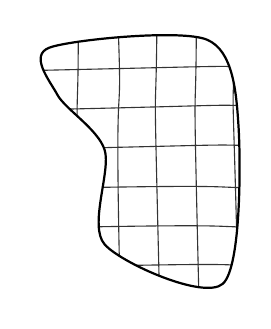
\begin{tikzpicture}
    \draw [thick] plot [smooth cycle] coordinates {(1.3, -1.2) (1.3, 0) (0.7, 0.7) (0.6, 1.3) (2.6, 1.4) (3, 0.3) (2.8, -1.7)};
    \clip plot [smooth cycle] coordinates {(1.3, -1.2) (1.3, 0) (0.7, 0.7) (0.6, 1.3) (2.6, 1.4) (3, 0.3) (2.8, -1.7)};
    \draw [step=0.5, opacity=0.8, decorate, decoration=penciline] (0, -2) grid (4, 1.7);
  \end{tikzpicture}
\end{center}
We then average out $X$ in each of these compartments to obtain $Y$. This is what we are going to call the conditional expectation of $X$ given $\mathcal{G}$, written $\E(X \mid \mathcal{G})$.

Ultimately, the characterizing property of $Y$ is the following lemma:
\begin{lemma} 
  The conditional expectation $Y = \E(X \mid \mathcal{G})$ satisfies the following properties:
  \begin{itemize}
    \item $Y$ is $\mathcal{G}$-measurable
    \item We have $Y \in L^1$, and
      \[
        \E Y \mathbf{1}_A = \E X \mathbf{1}_A
      \]
      for all $A \in \mathcal{G}$.
  \end{itemize}
\end{lemma}

\begin{proof}
  It is clear that $Y$ is $\mathcal{G}$-measurable. To show it is $L^1$, we compute
  \begin{align*}
    \E[|Y|] &= \E \left|\sum_{n = 1}^\infty \E(X \mid G_n) \mathbf{1}_{G_n}\right|\\
    &\leq \E \sum_{n =1 }^\infty \E(|X| \mid G_n) \mathbf{1}_{G_n} \\
    &= \sum \E \left( \E(|X| \mid G_n) \mathbf{1}_{G_n}\right)\\
    &= \sum \E |X| \mathbf{1}_{G_n}\\
    &= \E \sum |X| \mathbf{1}_{G_n}\\
    &= \E |X|\\
    &< \infty,
  \end{align*}
  where we used monotone convergence twice to swap the expectation and the sum.

  The final part is also clear, since we can explicitly enumerate the elements in $\mathcal{G}$ and see that they all satisfy the last property.
\end{proof}

It turns out for any $\sigma$-subalgebra $\mathcal{G} \subseteq \mathcal{F}$, we can construct the conditional expectation $\E(X \mid \mathcal{G})$, which is uniquely characterized by the above two properties.

\begin{thm}[Existence and uniqueness of conditional expectation]
  Let $X \in L^1$, and $\mathcal{G} \subseteq \mathcal{F}$. Then there exists a random variable $Y$ such that
  \begin{itemize}
    \item $Y$ is $\mathcal{G}$-measurable
    \item $Y \in L^1$, and $\E X \mathbf{1}_A = \E Y \mathbf{1}_A$ for all $A \in \mathcal{G}$.
  \end{itemize}
  Moreover, if $Y'$ is another random variable satisfying these conditions, then $Y' = Y$ almost surely.

  We call $Y$ a (version of) the conditional expectation given $\mathcal{G}$.
\end{thm}

We will write the condition expectation as $\E(X \mid \mathcal{G})$, and if $X = \mathbf{1}_A$, we will write $\E(A \mid \mathcal{G}) = \E(\mathbf{1}_A \mid \mathcal{G})$.

Recall also that if $Z$ is a random variable, then $\sigma(Z) = \{Z^{-1}(B): B \in \mathcal{B}\}$. In this case, we will write $\E[X \mid Z) = \E(X \mid \sigma(Z))$.

By, say, bounded convergence, it follows from the second condition that $\E XZ = \E YZ$ for all bounded $\mathcal{G}$-measurable functions $Z$.
\begin{proof}
  We first consider the case where $X \in L^2(\Omega, \mathcal{F}, \mu)$. Then we know from functional analysis that for any $\mathcal{G} \subseteq \mathcal{F}$, the space $L^2(\mathcal{G})$ is a Hilbert space with inner product
  \[
    \langle X, Y \rangle = \mu (X Y).
  \]
  In particular, $L^2(\mathcal{G})$ is a closed subspace of $L^2(\mathcal{F})$. We can then define $Y$ to be the orthogonal projection of $X$ onto $L^2(\mathcal{G})$. It is immediate that $Y$ is $\mathcal{G}$-measurable. For the second part, we use that $X - Y$ is orthogonal to $L^2(\mathcal{G})$, since that's what orthogonal projection is supposed to be. So $\E(X - Y)Z = 0$ for all $Z \in L^2(\mathcal{G})$. In particular, since the measure space is finite, the indicator function of any measurable subset is $L^2$. So we are done.

  We next focus on the case where $X \in m\mathcal{E}^+$. We define
  \[
    X_n = X \wedge n
  \]
  We want to use monotone convergence to obtain our result. To do so, we need the following result:

  \begin{claim}
    If $(X, Y)$ and $(X', Y')$ satisfy the conditions of the theorem, and $X' \geq X$ a.s., then $Y' \geq Y$ a.s.
  \end{claim}

  \begin{proof}
    Define the event $A = \{Y' \leq Y\} \in \mathcal{G}$. Consider the event $Z = (Y - Y')\mathbf{1}_A$. Then $Z \geq 0$. We then have
    \[
      \E Y' \mathbf{1}_A = \E X' \mathbf{1}_A \geq \E X \mathbf{1}_A = \E Y \mathbf{1}_A.
    \]
    So it follows that we also have $\E(Y - Y')\mathbf{1}_A \leq 0$. So in fact $\E Z = 0$. So $Y' \geq Y$ a.s.
  \end{proof}
  We can now define $Y_n = \E(X_n \mid \mathcal{G})$, picking them so that $\{Y_n\}$ is increasing. We then take $Y_\infty = \lim Y_n$. Then $Y_\infty$ is certainly $\mathcal{G}$-measurable, and by monotone convergence, if $A \in \mathcal{G}$, then
  \[
    \E X \mathbf{1}_A = \lim \E X_n \mathbf{1}_A = \lim \E Y_n \mathbf{1}_A = \E Y_\infty \mathbf{1}_A.
  \]
  Now if $\E X < \infty$, then $\E Y_\infty = \E X < \infty$. So we know $Y_\infty$ is finite a.s., and we can define $Y = Y_\infty \mathbf{1}_{Y_\infty < \infty}$.

  Finally, we work with arbitrary $X \in L^1$. We can write $X = X^+ - X^-$, and then define $Y^\pm = \E (X^\pm \mid \mathcal{G})$, and take $Y = Y^+ - Y^-$.

  Uniqueness is then clear.
\end{proof}

\begin{lemma}
  If $Y$ is $\sigma(Z)$-measurable, then there exists $h: \R \to \R$ Borel-measurable such that $Y = h(Z)$. In particular,
  \[
    \E(X \mid Z) = h(Z) \text{ a.s.}
  \]
  for some $h: \R \to \R$.
\end{lemma}
We can then define $\E(X \mid Z = z) = h(z)$. The point of doing this is that we want to allow for the case where in fact we have $\P(Z = z) = 0$, in which case our original definition does not make sense.

\begin{ex}
  Consider $X \in L^1$, and $Z: \Omega \to \N$ discrete. Compute $\E(X \mid Z)$ and compare our different definitions of conditional expectation.
\end{ex}

\begin{eg}
  Let $(U, V) \in \R^2$ with density $f_{U, V}(u, v)$, so that for any $B_1, B_2 \in \mathcal{B}$, we have
  \[
    \P(U \in B_1, V \in B_2) = \int_{B_1} \int_{b_2} f_{U, V}(u, v) \;\d u \;\d v.
  \]
  We want to compute $\E(h(V) \mid U)$, where $h: \R \to \R$ is Borel measurable. We can define
  \[
    f_U(u) = \int_\R f_{U, V} (u, v) \;\d v,
  \]
  and we define the conditional density of $V$ given $U$ by
  \[
    F_{ \mid U} (v \mid u) = \frac{f_{U, V}(u, v)}{f_U(u)}.
  \]
  We define
  \[
    g(u) = \int h(u) f_{V \mid U} (v \mid u)\;\d v.
  \]
  We claim that $\E(h(V) \mid U)$ is just $g(U)$.

  To check this, we show that it satisfies the two desired conditions. It is clear that it is $\sigma(U)$-measurable. To check the second condition, fix an $A \in \sigma(U)$. Then $A = \{(u, v): u \in B\}$ for some $B$. Then
  \begin{align*}
    \E(h(V) \mathbf{1}_A) &= \int \int h(v) \mathbf{1}_{u \in B} f_{U, V} (u, v)\;\d u\;\d v\\
    &= \int \int h(v) \mathbf{1}_{u \in B} f_{V \mid U}(v \mid u) f_V(u)\;\d u\;\d v\\
    &= \int g(U) \mathbf{1}_{u \in B} f_U(u) \;\d u\\
    &= \E(g(U) \mathbf{1}_A),
  \end{align*}
  as desired.
\end{eg}
The point of this example is that to compute conditional expectations, we use our intuition to guess what the conditional expectation should be, and then check that it satisfies the two uniquely characterizing properties.

\begin{eg}
  Suppose $(X, W)$ are Gaussian. Then for all linear functions $\varphi: \R^2 \to \R$, the quantity $\varphi(X, W)$ is Gaussian.

  One nice property of Gaussians is that lack of correlation implies independence. We want to compute $\E(X \mid W)$. Note that if $Y$ is such that $\E X = \E Y$, $X - Y$ is independent of $W$, and $Y$ is $W$-measurable, then $Y = \E(X \mid W)$, since
  $\E(X - Y) \mathbf{1}_A = 0$ for all $\sigma(W)$-measurable $A$.

  The guess is that we want $Y$ to be a Gaussian variable. We put $Y = aW + b$. Then $\E X = \E Y$ implies we must have
  \[
    a \E W + b = \E X.\tag{$*$}
  \]
  The independence part requires $\cov(X - Y, W) = 0$. Since covariance is linear, we have
  \[
    0 = \cov(X - Y, W) = \cov(X, W) - \cov(aW + b, W) = \cov(X, W) - a \cov(W, W).
  \]
  Recalling that $\cov(W, W) = \var(W)$, we need
  \[
    a = \frac{\cov(X, W)}{\var(W)}.
  \]
  This then allows us to use $(*)$ to compute $b$ as well. This is how we compute the conditional expectation of Gaussians.
\end{eg}

We note some immediate properties of conditional expectation. As usual, all (in)equality and convergence statements are to be taken with the quantifier ``almost surely''.
\begin{prop}\leavevmode
  \begin{enumerate}
    \item $\E(X \mid \mathcal{G}) = X$ iff $X$ is $\mathcal{G}$-measurable.
    \item $\E(\E(X \mid \mathcal{G})) = \E X$
    \item If $X \geq 0$ a.s., then $\E(X \mid \mathcal{G}) \geq 0$
    \item If $X$ and $\mathcal{G}$ are independent, then $\E(X \mid \mathcal{G}) = \E[X]$
    \item If $\alpha, \beta \in \R$ and $X_1, X_2 \in L^1$, then
      \[
        \E(\alpha X_1 + \beta X_2 \mid \mathcal{G}) = \alpha \E(X_1 \mid\mathcal{G}) + \beta \E(X_2 \mid \mathcal{G}).
      \]
    \item Suppose $X_n \nearrow X$. Then
      \[
        \E(X_n\mid \mathcal{G}) \nearrow \E(X \mid \mathcal{G}).
      \]
    \item \term{Fatou's lemma}: If $X_n$ are non-negative measurable, then
      \[
        \E\left(\liminf_{n \to \infty} X_n \mid \mathcal{G}\right) \leq \liminf_{n \to \infty} \E(X_n \mid \mathcal{G}).
      \]
    \item \emph{Dominated convergence theorem}\index{dominated convergence theorem}: If $X_n \to X$ and $Y \in L^1$ such that $Y \geq |X_n|$ for all $n$, then
      \[
        \E(X_n \mid \mathcal{G}) \to \E(X \mid \mathcal{G}).
      \]
    \item \term{Jensen's inequality}: If $c: \R \to \R$ is convex, then
      \[
        \E(c(X) \mid \mathcal{G}) \geq c(\E(X) \mid \mathcal{G}).
      \]
    \item \emph{Tower property}\index{tower property}: If $\mathcal{H} \subseteq \mathcal{G}$, then
      \[
        \E(\E(X \mid \mathcal{G}) \mid \mathcal{H}) = \E(X \mid \mathcal{H}).
      \]
    \item
      \[
        \|\E(X \mid \mathcal{G}\|_p \leq \|X\|_p.
      \]
    \item If $Z$ is bounded and $\mathcal{G}$-measurable, then
      \[
        \E(ZX \mid \mathcal{G}) = Z \E(X \mid \mathcal{G}).
      \]
    \item Let $X \in L^1$ and $\mathcal{G}, \mathcal{H} \subseteq \mathcal{F}$. Assume that $\sigma(X, \mathcal{G})$ is independent of $\mathcal{H}$. Then
      \[
        \E (X \mid \mathcal{G}) = \E(X \mid \sigma(\mathcal{G}, \mathcal{H})).
      \]
  \end{enumerate}
\end{prop}

\begin{proof}
  \begin{enumerate} % actually check these
    \item Clear.
    \item Take $A = \omega$.
    \item Shown in the proof.
    \item Clear by property of expected value of independent variables.
    \item Clear, since the RHS satisfies the unique characterizing property of the LHS.
    \item Clear from construction.
    \item Same as the unconditional proof, using the previous property.
    \item Same as the unconditional proof, using the previous property.
    \item Same as the unconditional proof.
    \item The LHS satisfies the characterizing property of the RHS
    \item Using the convexity of $x^p$, Jensen's inequality tells us
      \begin{align*}
        \|E(X \mid \mathcal{G})\|_p^p &= \E |\E(X \mid \mathcal{G})|^p\\
        &\leq \E (\E (|X|^p \mid \mathcal{G}))\\
        &= \E |X|^p\\
        &= \|X\|_p^p
      \end{align*}
    \item If $Z = \mathbf{1}_B$, and let $b \in \mathcal{G}$. Then
      \[
        \E(Z \E(X \mid \mathcal{G}) \mathbf{1}_A) = \E (\E (X \mid \mathcal{G}) \cdot \mathbf{1}_{A \cap B}) = \E(X \mathbf{1}_{A \cap B}) = \E(Z X \mathbf{1}_A).
      \]
      So the lemma holds. Linearity then implies the result for $Z$ simple, then apply our favorite convergence theorems.
    \item Take $B \in \mathcal{H}$ and $A \in \mathcal{G}$. Then
      \begin{align*}
        \E(\E(X \mid \sigma(\mathcal{G}, \mathcal{H}))\cdot \mathbf{1}_{A \cap B}) &= \E(X \cdot \mathbf{1}_{A \cap B})\\
        &= \E(X \mathbf{1}_A) \P(B)\\
        &= \E(\E(X \mid \mathcal{G}) \mathbf{1}_A) \P(B)\\
        &= \E(\E(X \mid \mathcal{G}) \mathbf{1}_{A \cap B})
      \end{align*}
      If instead of $A \cap B$, we had any $\sigma(\mathcal{G}, \mathcal{H})$-measurable set, then we would be done. But we are fine, since the set of subsets of the form $A \cap B$ with $A \in \mathcal{G}$, $B \in \mathcal{H}$ is a generating $\pi$-system for $\sigma(\mathcal{H}, \mathcal{G})$.
  \end{enumerate}
\end{proof}
The proofs are either straightforward, already present in the proof above, or has the same proof as the non-conditional cases.

\begin{lemma}
  If $X \in L^1$, then the family of random variables $Y_{\mathcal{G}} = \E(X \mid \mathcal{G})$ for all $\mathcal{G} \subseteq \mathcal{F}$ is uniformly integrable.

  In other words, for all $\varepsilon > 0$, there exists $\lambda > 0$ such that
  \[
    \E(Y_{\mathcal{G}} \mathbf{1}_{|Y_{\mathcal{G}} > \lambda|}) < \varepsilon
  \]
  for all $\mathcal{G}$.
\end{lemma}

\begin{proof}
  Fix $\varepsilon > 0$. Then there exists $\delta > 0$ such that $\E |X|\mathbf{1}_A < \varepsilon$ for any $A$ with $\P(A) < \delta$.

  Take $Y = \E (X \mid \mathcal{G})$. Then $|Y| \leq \E(|x| \mid \mathcal{G})$. In particular,
  \[
    \E|Y| \leq \E|X|.
  \]
  By Markov's inequality, we have
  \[
    \P(|Y| \geq \lambda) \leq \frac{\E|Y|}{\lambda} \leq \frac{\E|X|}{\lambda}.
  \]
  So take $\lambda$ such that $\frac{\E|X|}{\lambda} < \delta$. So we have
  \[
    \E(|Y| \mathbf{1}_{\{|Y| \geq \lambda\}}) \leq \E(\E(|X| \mid \mathcal{G})\mathbf{1}_{|Y| \geq \lambda})
  \]
  But $\mathbf{1}_{|Y| \geq \lambda}$ is a $\mathcal{G}$-measurable function. So this is equal to
  \[
    \E(|X| \mathbf{1}_{\{Y| \geq \lambda}\}) < \varepsilon.
  \]
\end{proof}

\section{Martingales in discrete time}

We again have $(\Omega, \mathcal{F}, \P)$.

\begin{defi}[Filtration]\index{filtration}
  A \emph{filtration} is a sequence of $\sigma$-algebras $(\mathcal{F}_n)_{n \geq 0}$ such that $\mathcal{F} \supseteq \mathcal{F}_{n + 1} \supseteq \mathcal{F}_n$. We define $\mathcal{F}_\infty = \sigma(\mathcal{F}_0, \mathcal{F}_1, \ldots) \subseteq \mathcal{F}$.
\end{defi}

This is supposed to model the evolution of time, where $\mathcal{F}_n$ consists of the information we have at time $t = n$. We will from now on assume $(\Omega, \mathcal{F}, \P)$ is equipped with a filtration $(\mathcal{F}_n)_{n \geq 0}$.

\begin{defi}[Stochastic process in discrete time]\index{discrete stochastic process}\index{stochastic process!discrete}
  A \emph{stochastic process} (in discrete time) is a sequence of random variables $(X_n)_{n \geq 0}$.
\end{defi}

\begin{defi}[Natural filtration]\index{natural filtration}\index{filtration!natural}
  The \emph{natural filtration} of $(X_n)_{n \geq 0}$ is given by
  \[
    \mathcal{F}_n^X  = \sigma(X_1, \ldots, X_n).
  \]
\end{defi}

\begin{defi}[Adapted process]\index{adapted process}\index{stochastic process!adapted}
  We say that $(X_n)_{n \geq 0}$ is \emph{adapted} (to $(\mathcal{F}_n)_{n \geq 0}$) if $X_n$ is $\mathcal{F}_n$-measurable for all $n \geq 0$.

  This is equivalent to saying that $\mathcal{F}^X_n \subseteq \mathcal{F}_n$.
\end{defi}

\begin{defi}[Integrable process]\index{integrable process}\index{stochastic process!integrable}
  A process $(X_n)_{n \geq 0}$ is \emph{integrable} if $X_n \in L^1$ for all $n \geq 0$.
\end{defi}

\begin{defi}[Martingale]\index{martingale}
  An integrable adapted process $(X_n)_{n \geq 0}$ is a \emph{martingale} if for all $m \leq n$, we have
  \[
    \E(X_n \mid \mathcal{F}_m) = X_m.
  \]
  We say it is a \term{super-martingale} if
  \[
    \E(X_n \mid \mathcal{F}_m) \leq X_m,
  \]
  and a \term{sub-martingale} if
  \[
    \E(X_n \mid \mathcal{F}_m) \geq X_m,
  \]
\end{defi}

Note that it is enough to take $m = n - 1$ for all $n \geq 0$, using the tower property.

\subsection{Stopping time and optimal stopping}

\begin{defi}[Stopping time]\index{stopping time}
  A \emph{stopping time} is a random variable $T: \Omega \to \N_{ \geq 0} \cup \{\infty\}$ such that
  \[
    \{T \leq n\} \in \mathcal{F}_n
  \]
  for all $n \geq 0$.
\end{defi}
This means to know that at time $n$, if we want to know if $T$ has come, we can determine it using the information we have at $T$.

\begin{eg}
  If $B \in \mathcal{B}(\R)$, then we can define
  \[
    T = \inf \{n : X_n \in B\}.
  \]
  Then this is a stopping time.

  On the other hand,
  \[
    T = \sup \{n: X_n \in B\}
  \]
  is not a stopping time (in general).
\end{eg}

\begin{defi}[$\mathcal{F}_T$]\index{$\mathcal{F}_T$}
  For a stopping time $T$, define
  \[
    \mathcal{F}_T = \{A \in \mathcal{F}_\infty : A \cap \{T \leq n\} \in \mathcal{F}_n\}.
  \]
\end{defi}
One sees that this is a $\sigma$-algebra.

\begin{eg}
  If $T \equiv n$ is constant, then $F\mathcal{F}_T = \mathcal{F}_n$.
\end{eg}

\begin{defi}[$X_T$]\index{$X_T$}
  For a stopping time $T$, we define the random variable $X_T$ by
  \[
    X_T (\omega) = X_{T(\omega)}(\omega)
  \]
  on $\{T < \infty\}$, and $0$ otherwise.
\end{defi}

\begin{defi}[Stopped process]\index{stopped process}
  The \emph{stopped process} is defined by
  \[
    (X_n^T)_{n \geq 0} = (X_{T(\omega) \wedge n}(\omega))_{n \geq 0}.
  \]
\end{defi}
So we stop the process once $T$ happens.
\printindex
\end{document}
